% start the document

% specify the document layout and font size
\documentclass[preprint,12pt]{elsarticle}
\usepackage[margin=1.5cm,includefoot]{geometry}
\usepackage{setspace}

% uploading packages
\usepackage{graphicx}
\usepackage{amssymb}
\usepackage{gensymb}
\usepackage{lineno}
\usepackage{mathtools}
\usepackage{siunitx}
\usepackage[colorlinks]{hyperref}
\usepackage[nameinlink,capitalise]{cleveref} %needs to appear after hyperref, https://tex.stackexchange.com/questions/396728/my-equations-referencing-not-working
\Crefname{figure}{Figure}{Figures} %needs to appear after hyperref and cleveref
\newcommand\crefrangeconjunction{--} % modify the reference style
\usepackage{mathrsfs}
\usepackage{url}
\usepackage{enumitem}
\usepackage{tabulary}
\usepackage{multirow}
\graphicspath{{figures/}} %Setting the graphicspath
% ---------to deal with the double quotes----------- 
\usepackage [english]{babel}
\usepackage [autostyle, english = american]{csquotes}
\MakeOuterQuote{"}
%alternatively can use `` '' format for double quotes
\usepackage{booktabs}
\setlength{\abovetopsep}{1ex}
\usepackage[shortcuts,abbreviations,headuc]{glossaries-extra}
\newcommand*{\TCac}[1]{\ecapitalisewords{\glsentrylong{#1}}}

\glssetcategoryattribute{abbreviation}{indexonlyfirst}{true}
\glssetcategoryattribute{abbreviation}{nohyper}{true}
\makeglossaries

\newabbreviation{5dof}{5DOF}{five degree-of-freedom}
\newabbreviation{ebsd}{EBSD}{electron backscatter diffraction}
\newabbreviation[longplural={grain boundaries}]{gb}{GB}{grain boundary}
\newabbreviation{fcc}{FCC}{face-centered cubic}
\newabbreviation{mfc}{MFC}{mass flow controller}
\newabbreviation{sem}{SEM}{scanning electron microscope}
\newabbreviation{fea}{FEA}{finite element analysis}
\newabbreviation{bcs}{BCs}{boundary conditions}
\newabbreviation[longplural={triple junctions}]{tj}{TJ}{triple junction}
\newabbreviation{gpr}{GPR}{Gaussian process regression}
\newabbreviation{ann}{ANN}{artificial neural network}
\newabbreviation{nn}{NN}{nearest neighbor}
\newabbreviation{rmse}{RMSE}{root mean square error}
\newabbreviation{mae}{MAE}{mean absolute error}
\newabbreviation{brk}{BRK}{Bulatov Reed Kumar}
\newabbreviation{gbed}{GBED}{grain boundary energy distribution}
\newabbreviation{gbcd}{GBCD}{grain boundary character distribution}
\newabbreviation{mfz}{MFZ}{misorientation fundamental zone}
\newabbreviation{bp}{BP}{boundary plane}
\newabbreviation{knn}{kNN}{k-nearest neighbor}
\newabbreviation{gbe}{GBE}{grain boundary energy}
\newabbreviation{gbo}{GBO}{grain boundary octonion}
\newabbreviation{oslerp}{oSLERP}{octonion Spherical Linear Interpolation}
\newabbreviation{loocv}{LOOCV}{leave-one-out cross validation}
\newabbreviation{kfcv}{kFCV}{k-fold cross validation}
\newabbreviation{seo}{SEO}{symmetrically equivalent octonion}
\newabbreviation{fex}{FEX}{file exchange}
\newabbreviation{idw}{IDW}{inverse-distance weighting}
\newabbreviation{fic}{FIC}{fully independent conditional}
\newabbreviation{svd}{SVD}{singular value decomposition}
\newabbreviation{gbc}{GBC}{grain boundary character}
\newabbreviation{fz}{FZ}{fundamental zone}
\newabbreviation{pfz}{pFZ}{pseudo fundamental zone}
\newabbreviation{cmo}{CMO}{closed-mesh octonion}
\newabbreviation{lobpcg}{LOBPCG}{locally optimal block preconditioned conjugate gradient}
\newabbreviation{lkr}{LKR}{Laplacian kernel regression}
% example abbreviations
% \newabbreviation{seo}{SEO}{symmetrically equivalent octonions}
%\newabbreviation[longplural={grain boundaries}]{gb}{GB}{grain boundary}

%example usage: \gls{gpr}
%example usage: \Gls{gpr} (capitalize first letter, only meaningful for first usage)
% \glspl{seo} --> symmetrically equivalent octonions OR SEOs
%^^^^^^^^^^^^^^^^^^^^^^^^^^^^^^^^^^^^^^^^^^^^^^^^^^^


%\title{Grain Boundary Octonion Meshing and Interpolation}
\title{Five Degree-of-Freedom Property Interpolation of Arbitrary Grain Boundaries via \glsentrytitlecase{cmo}{long} Framework}
\author[myu]{Sterling G. Baird}
\author[myu]{Eric R. Homer}
\author[myu]{David T. Fullwood}
\author[myu]{Oliver K. Johnson\corref{cor1}}

\address[myu]{Department of Mechanical Engineering, Brigham Young University, Provo, UT 84602, USA}
\cortext[cor1]{Corresponding author}
\date{October 2020}

% Double Spacing
% \doublespacing
\begin{document}

\begin{abstract}
    In this work we introduce the \gls{cmo} interpolation framework for \gls{gb} structure-property models and surrogates. The \gls{cmo} framework offers an advantage over other \gls{5dof} based property interpolation methods because it is constructed as a closed mesh in a Riemannian manifold, for which Euclidean and arc length distances take on meaning and significantly reduce computation time compared with other distance metrics. This increased efficiency facilitates the use of significantly more input data and therefore leads to a reduction of the interpolation error. As a demonstration, we present \gls{gbe} interpolation results for a non-smooth validation function (Bulatov, Reed, Kumar) \cite{bulatovGrainBoundaryEnergy2014}.
    %and simulated bi-crystal datasets from the literature for Ni and Fe.
    Four interpolation methods built on this framework --- barycentric interpolation, \gls{gpr} or Kriging, \gls{idw}, and \gls{nn} interpolation --- are presented and compared against a constant, average model (\gls{rmse} $\simeq$ \SI{0.13}{\J\per\square\meter}), resulting in \gls{rmse} values of 0.063, 0.056, 0.068, and \SI{0.082}{\J\per\square\meter}, respectively, for \num{50000} randomly sampled input \glspl{gb} and evaluated for \num{10000} randomly sampled prediction \glspl{gb}. A vectorized, parallelized, MATLAB interpolation function is made available (\url{github.com/sgbaird-5dof/interp}). The \gls{cmo} framework offers a great advantage in estimating property values for arbitrary \glspl{gb} and modeling surrogates of computationally expensive \gls{5dof} functions and simulations.
\end{abstract}

% 2020-10-24  The closed-octonion interpolation framework offers an advantage over other five-degree-of-freedom based property interpolation methods because it's defined as a closed mesh in a Riemannian manifold. One can triangulate a mesh using standard routines (e.g. quickhull, qhull.org) and interpolate using barycentric coordinates or machine learning methods such as Gaussian Process Regression. Euclidean and arc length distances take on meaning in this framework and are trivial computations compared with other distance metrics, thereby addressing a limitation in previous work. The ability to use significantly more input data lends itself to lower interpolation error and is demonstrated by grain boundary energy interpolation results for a non-smooth validation function (Bulatov, Reed, Kumar) and simulated bi-crystal datasets from the literature for Ni and Fe. Four interpolation methods built on this framework --- barycentric interpolation, Gaussian Process Regression or Kriging, inverse-distance weighting, nearest neighbor interpolation --- are presented and compared against a constant, average model (RMSE = 0.013 \J\per\square\meter), resulting in RMSE values of 0.063, 0.056, 0.068, and 0.082 \J\per\square\meter, respectively, for \num{50000} randomly input sampled bicrystals and evaluated for \num{10000} randomly sampled output bicrystals. A vectorized, parallelized, MATLAB implementation is made available (github.com/sgbaird-5dof/interp) with similar input/output structure of built-in MATLAB interpolation functions (e.g. \textit{interpn}) and placeholders for custom interpolation schemes. The closed-octonion framework offers a great advantage in estimating property values for arbitrary grain boundaries based on experimental or simulated data and modeling surrogates of computationally expensive 5DOF functions and simulations.

\maketitle

\section{Introduction} \label{sec:intro}

In this work, we present a new method for interpolation and prediction of grain boundary (GB) properties from a set of measured/calculated values. Our approach, called the \gls{cmo} framework is highly efficient, and thereby facilitates the use of large data sets to enhance prediction accuracy.

\subsection{Previous Work}
In previous work, a number of strategies have been developed for describing a \gls{5dof} \gls{gb} property based on experimental or simulated data. Binning and gradient descent were used to produce a \gls{5dof} \gls{gbed} in nickel \cite{liRelativeGrainBoundary2009}, yttria \cite{dillonCharacterizationGrainboundaryCharacter2009}, and copper \cite{randleFiveparameterGrainBoundary2008} based on experimentally characterized 3D microstructures. 

A non-discretizing approach was recently introduced \cite{shenDeterminingGrainBoundary2019} that utilizes regularization imposed on \gls{tj} equilibrium equations, the \gls{lobpcg} method, and \gls{knn} distances. In this approach, \num{60000} \glspl{tj} and a custom, non-smooth validation function are used to obtain \gls{gbe} \gls{rmse} values of approximately \SI{0.01}{\J\per\square\meter} and \SI{0.03}{\J\per\square\meter} for \gls{gbe} values less than \SI{0.9}{\J\per\square\meter} and greater than \SI{0.9}{\J\per\square\meter}, respectively. 

\citet{echeverrirestrepoUsingArtificialNeural2014} used an \gls{ann} and approximately \num{17000} and \num{51000} Fe bicrystal simulations from \citet{kimIdentificationSchemeGrain2011} as training and validation data, respectively, to achieve \glspl{mae} of approximately \SI{0.05}{\J\per\square\meter} and \SI{0.09}{\J\per\square\meter} in the best fitted \glspl{ann} for randomly selected and special \glspl{gb}, respectively. 

Recently, a new \gls{gb} representation termed \glspl{gbo} was reported \cite{francisGeodesicOctonionMetric2019} and tested \cite{chesserLearningGrainBoundary2020}. The \gls{gbo} representation is valuable for a number of applications. Most relevant to the present work is the resulting distance metric. The \gls{gbo} distance metric offers an advantage over other metrics in that it "correctly determines the angular distances between \glspl{gb} with a common normal or misorientation" and "closely approximates the geodesic metric on $SO(3) \times SO(3)$ \textit{for all grain boundary pairs} while maintaining the ability to be analytically minimized with respect to the $U(1)$ symmetry" \cite{francisGeodesicOctonionMetric2019}. In this context, \citet{francisGeodesicOctonionMetric2019} derived \gls{oslerp} and provided examples showing that \gls{oslerp} produces smooth, minimum distance paths through \gls{gb} character space between two arbitrary \glspl{gb}. 

\Gls{lkr} (a type of \gls{idw}) involving scaled pairwise distance matrices were later used with \gls{gbo}s to predict properties of arbitrary \glspl{gb} from a set of known values \cite{chesserLearningGrainBoundary2020}. Using \gls{kfcv} with $k=10$ for \num{388} Ni \gls{gbe} simulations \cite{holmComparingGrainBoundary2010} and an optimized scaling parameter, an \gls{rmse} of \SI{0.0977}{\J\per\square\meter} was obtained. Due to computation time of pairwise distance matrices, this approach is limited to datasets with several thousand \glspl{gb} or fewer \cite{chesserLearningGrainBoundary2020}.

\subsection{\glsentrytitlecase{cmo}{long} Framework}
The \gls{cmo} interpolation framework introduced in this work offers an advantage over other methods because it is defined as a closed mesh in a Riemannian manifold. This is evidenced by the ability to triangulate a mesh using standard routines (e.g. quickhull \cite{barberQuickhullAlgorithmConvex1996}) and interpolate using barycentric coordinates or machine learning methods such as \gls{gpr}. Building on previous work on \glspl{gbo} \cite{francisGeodesicOctonionMetric2019,chesserLearningGrainBoundary2020}, we obtain a closed mesh by obtaining a set of octonions minimized with respect to Euclidean distance and an arbitrary reference octonion after considering all \glspl{seo}. Because \glspl{gbo} are guaranteed to reside on the surface of a hypersphere \cite{francisGeodesicOctonionMetric2019} (a type of Riemannian manifold) a closed mesh is thus formed which locally resembles Euclidean space (\cref{sec:methods:closed-mesh-comparison}). Below we mention a few benefits and applications of this approach, after which we provide the detailed description of the method (\cref{sec:methods}) and numerical test results (\cref{sec:results}).

\subsection{Benefits of \glsentrytitlecase{cmo}{long} Framework}
\subsubsection{Distance Calculations}
Because Euclidean and arc length distances take on meaning in this framework, distance computations are much faster than other metrics. The calculation speed is even higher than explicit \gls{gbo} distance calculations using the original octonion distance given in \cite{francisGeodesicOctonionMetric2019}. For example, a \num{50000} x \num{50000} pairwise-distance matrix can be computed in approximately 10 s using built-in MATLAB \textit{Statistics and Machine Learning Toolbox} function \texttt{pdist} -- something that was computationally challenging before and a limitation of previous work. Compared to the original octonion metric, this represents an improvement in computational speed by several orders of magnitude. This is due to the fact that \glspl{seo} only need to be considered once per \gls{gb}, $O(N_p^2L^2)$, rather than once per distance calculation 
%per \gls{gb} in a \gls{gb}-pair
, $O(N_p^4L^2)$, where $N_p$ is the symmetry cardinality ($N_p=24$ for $m\Bar{3}m$ \gls{fcc} point group) and $L$ is the number of \glspl{gb}. % $O(N^2L)$ (this work) vs. $O(N^4L^2$ (octonion paper)

\subsubsection{Interpolation Error}
The ability to use significantly more input data lends itself to lower interpolation error. This will be demonstrated by \gls{gbe} interpolation results for a non-smooth validation function in \cref{sec:results}.
%and simulated bi-crystal datasets from the literature (388 Olmsted Ni \cite{olmstedSurveyComputedGrain2009} and \num{50000} Kim Fe \cite{kimIdentificationSchemeGrain2011} bicrystals).
Four interpolation methods built on this framework --- barycentric (\cref{sec:methods:bary}), \gls{gpr} or Kriging (\cref{sec:methods:gpr}), \gls{idw} (\cref{sec:methods:idw}), \gls{nn} (\cref{sec:methods:nn}) --- will be presented and compared against a constant, average model (\cref{sec:results}). To facilitate easy application of the presented method, a vectorized, parallelized, MATLAB implementation, \texttt{interp5DOF}, is made available \cite{bairdFiveDegreeofFreedom5DOF2020} with similar input/output structure to that of the built-in MATLAB interpolation functions (e.g. \texttt{interpn()}) and placeholders for custom interpolation schemes. A typical function call is as follows: \texttt{ypred = interp5DOF(qm,nA,propList,qm2,nA2,method)}. Input misorientation quaternions (e.g. \texttt{qm}) and \gls{bp} normals (e.g. \texttt{nA}) define the mesh (\texttt{qm}, \texttt{nA}) and prediction or query points (\texttt{qm2}, \texttt{nA2}). Property values (\texttt{propList}) of \glspl{gb} corresponding to the \texttt{qm}/\texttt{nA} pairs are supplied. Interpolated or predicted values (\texttt{ypred}) corresponding to the \texttt{qm2}/\texttt{nA2} pairs are returned. The methods (\texttt{method}) used in this work are \texttt{'pbary'}, \texttt{'gpr'}, \texttt{'idw'}, and \texttt{'nn'}, corresponding to planar barycentric, \gls{gpr}, \gls{idw}, and \gls{nn} interpolation, respectively, and a placeholder template with instructions is provided in \texttt{interp5DOF}. Misorientation quaternions are represented in the active sense:
\begin{equation}
    q_m = {q_A}^{-1}q_B
\end{equation}
where $q_m$, $q_A$, and $q_B$ represent the misorientation quaternion, quaternion of grain A in the sample frame, and quaternion of grain B in the sample frame, respectively. The $^{-1}$ operator denotes a quaternion inverse. \Gls{bp} unit normals are expressed pointing away from grain A and in the reference frame of grain A (i.e. the outward-pointing normal convention).

\subsubsection{Applications}

The \gls{cmo} framework offers a great advantage in estimating property values for arbitrary \glspl{gb} based on experimental or simulated data such as energy, mobility, and diffusivity. The framework can also enable efficient surrogate modeling of computationally expensive 5DOF functions and simulations such as in evaluation of the \gls{brk} function for use in anisotropic grain growth simulations. In other words, one can evaluate the CMO surrogate model in a fraction of the time of the true property model, thereby facilitating larger scale iterative simulations, which require repetitive evaluation of a computationally expensive structure-property model.

\section{Methods} \label{sec:methods}

The core operations of the \gls{cmo} framework are (i) the calculation of, and (ii) projection of points into, a \gls{gb} \gls{fz}, (iii) the triangulation of the \gls{fz} (for barycentric interpolation), and (iv) distance calculations within the \gls{fz}. Rather than relying on an analytically defined \gls{fz}, we employ a numerical approximation, which we will refer to as a \gls{pfz}.

The construction of the \gls{pfz} dramatically reduces the computational burden of pairwise distance calculations. The mechanism by which this reduction is achieved can best be illustrated with an example. Let $o_1$ and $o_2$ denote two \glspl{gb} represented as octonions, or \glspl{gbo}. 

To perform a traditional distance calculation it is necessary to compare all \glspl{seo} of $o_1$ to all of the \glspl{seo} of $o_2$ and take the smallest distance. If $N_p$ is the cardinality of the crystallographic point group, this single minimum distance calculation requires a total of $N_p^4$ intermediate distance calculations. If one desires to compute a pairwise distance matrix between $L$ GBs, the total computational cost will be $O(N_p^4L^2)$.

In contrast, for a single distance calculation using the \gls{cmo} framework, $o_1$ and $o_2$ are first projected into the \gls{pfz}, and then only a single distance calculation is required between them. Projecting $o_1$ into the \gls{pfz} requires comparison of all $N_p^2$ \glspl{seo} of $o_1$ with a fixed reference \gls{gb} in the interior of the \gls{pfz}; and likewise for $o_2$. Consequently, a single distance calculation between $o_1$ and $o_2$ under the \gls{cmo} framework requires $2N_p^2$ intermediate distance calculations. If one desires to compute a pairwise distance matrix between $L$ \glspl{gb}, the total computational cost will be $O(N_p^2L^2)$, which represents a dramatic reduction. A summary of the differences between the two approaches is provided in \cref{tab:closed-mesh-comparison}.

\begin{table}
\caption{Comparison between \acrlong{cmo} and traditional octonion frameworks. *6D Cartesian representation used only for mesh triangulation efficiency in barycentric interpolation and *7D Cartesian representation only required for barycentric interpolation. For pairwise distance complexity, $N_p$ is the symmetry cardinality ($N_p=24$ for $m\Bar{3}m$ \gls{fcc} point group) and $L$ is the number of \glspl{gb}.}
\centering
\begin{tabular}{ccc}
\toprule
Property & Traditional & This Work \\
\midrule
Symmetrizing Distance & Octonion & Euclidean \\
Considered \glspl{seo} & Subset & All \\
Dimensionality & 8D Cartesian & 6*/7*/8D Cartesian \\
Riemannian Mesh & No & Yes \\
% Euclidean Approximation Valid & No & Yes \\
Pairwise Distance Complexity & $O(N_p^4L^2)$ & $O(N_p^2L^2)$ \\
\bottomrule
\end{tabular}
\label{tab:closed-mesh-comparison}
\end{table}

In this section we describe our methods for each of the \gls{cmo} framework operations (i)-(iv) named above. We then describe our implementation of 4 different interpolation schemes for prediction of GB properties based on the \gls{cmo} approach.

\subsection{The \glsentrytitlecase{cmo}{long} Framework}
\label{sec:methods:framework}

\subsubsection{Defining the \glsentrytitlecase{pfz}{long}}
\label{sec:methods:pFZ}

% Explain the "voronoi" type definition of the pFZ by choosing a reference GB and then taking the symmetric image of each GB that is closest to that reference GB. You will need to convince the reader (probably by reason, or proof, or numerical tests) that the resulting pFZ does in fact contain one and ONLY one SEO for every GB (i.e. that it does satisfy the definition of a FZ). This is probably where you note that for it to work, the reference GB needs to be something that isn't a high-symmetry GB, and why. This discussion will probably benefit from a figure illustrating the procedure in 2D.


a unique octonion is found within numerical tolerance as long as the reference \gls{gbo} is low-symmetry (very likely based on random sampling and can be verified).

Because a fixed, arbitrary, reference octonion is used to symmetrize the mesh, meshes with different exterior bounds can be obtained based on the reference octonion used. This is a limitation of this work in that the boundaries of the mesh do not correspond with high-symmetry \glspl{gb} in contrast with typical \gls{fz} representations in misorientation or \gls{bp} \cite{patalaSymmetriesRepresentationGrain2013,homerGrainBoundaryPlane2015} spaces. Interpolated values near the exterior of the mesh are likely to have higher error because the local region of influence may be prematurely cut off for \gls{gpr} and \gls{idw}. By definition of the barycentric and \gls{nn} methods, extrapolation is necessary to predict values on or near the "true" boundary of the mesh due to expected curvature in those boundaries. Further, \gls{nn} and barycentric interpolation are the only two non-smooth interpolation methods used; in these two cases, sharp cusps in the model will be smoothed or misrepresented unless there are \glspl{gb} on the cusp. For \gls{gpr} and \gls{idw}, cusps will be smoothed by definition as long as there is a non-zero kernel and non-zero standard deviation employed. This is a feature common to previously published methods \cite{liRelativeGrainBoundary2009,shenDeterminingGrainBoundary2019,chesserLearningGrainBoundary2020} except for those \cite{bulatovGrainBoundaryEnergy2014,shekhawatGeneralizedReadShockley2016} which explicitly implement the Read-Shockley model \cite{readDislocationModelsCrystal1950}. For a discussion of possible ways to address these issues, see Section \cref{sec:conclusions:future}.


\subsubsection{Projecting \glsentrypltitlecase{gb}{long} to the \glsentrytitlecase{pfz}{long}}
\label{sec:methods:projecting}

% With the reference GB chosen, and consequently the pFZ defined, explain that a GB is projected into the pFZ simply by finding among its \glspl{seo} the one that is closest to the reference GB.

\subsubsection{Triangulation of the \glsentrytitlecase{pfz}{long}}
\label{sec:methods:triangulation}

% Briefly (but clearly and explicitly) explain the steps of generating the cubochorically sampled GBs, converting them to octonions and then projecting all of them into the pFZ. Then explain how you do the triangulation. This will require a few figures to show the process in 3D (i.e. generating a triangulation of a point cloud on a region of the surface of the 2-sphere).

\subsubsection{Distance Calculations in the \glsentrytitlecase{pfz}{long}}
\label{sec:methods:distancepFZ}

% Explain how to compute distances in the pFZ, and why you can now just use euclidean distances.

\subsection{Interpolation in the \glsentrytitlecase{cmo}{long} Framework}
\label{sec:methods:interpolation}

\subsubsection{Barycentric Interpolation}
\label{sec:methods:bary}

% Give brief explanation of standard barycentric interpolation: you find which simplex the point is in, then you calculate the weights. The advantage of this approach is that the weight matrix only has to be computed once. If you interpolate different functions over the same query points, the weights don't change, so re-evaluation with a new function is rapid via a simple matrix multiplication.

% Explain how to adapt barycentric interpolation to the pFZ: how to identify which simplex the query point falls in, and then how to compute the weights. Also explain and justify why you can use euclidean distances (i.e. because the pFZ occupies a small portion of the 7-sphere it is nearly planar so euclidean distances and octonion distances are approximately equal and you can show tha figure here), and how that speeds things up.

While spherical-arc-length-preserving methods were implemented and tested, only default interpolation methods using Euclidean distances are reported in this work. This is because Euclidean distances are a close approximation to spherical arc length for symmetrized octonions in a closed-mesh (\cref{fig:dist-parity} and use of Euclidean distance enables a wider range of built-in methods and routines and is faster to compute. For example, in the case of \gls{gpr}, due a limited selection of analytical derivatives, the MATLAB built-in function \textit{fitrgp} is approximately two orders of magnitude slower when using a custom octonion distance rather than the built-in Euclidean distance despite producing nearly identical results.

\begin{figure}
\centering
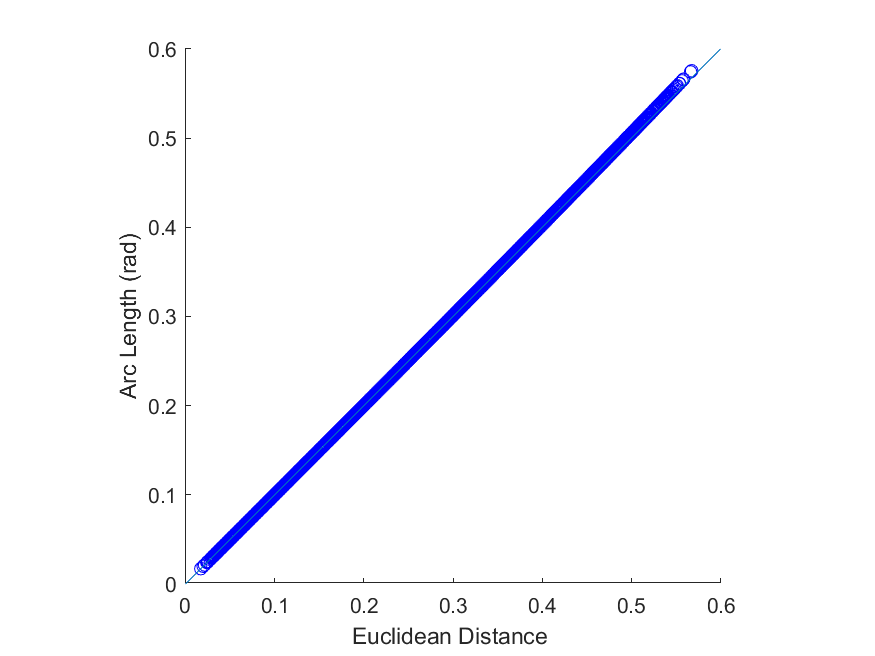
\includegraphics[width=0.5\linewidth]{dist-parity.png}
\caption{Parity plot of hyperspherical arc length vs. Euclidean distance for pairwise distances in a symmetrized, closed-mesh of \num{10000} randomly sampled \acrlongpl{gbo}. The max arc length is approximately \SI{0.58}{\radian}, indicating a max octonion distance of approximately \SI{1.16}{\radian} or \SI{66.5}{\degree} between any two points in the \acrlong{fz}. The close correlation between arc length and Euclidean distance supports the validity of using Euclidean distance in the interpolation methods.}
\label{fig:dist-parity}
\end{figure}

\subsubsection{\glsentrytitlecase{gpr}{long}}

% You don't need to give a detailed explanation of GPR, but you do need 1 sentence summarizing the idea and then point to REF for a general treatment. Explain any assumptions or adaptations that need to be done to use it with the pFZ (e.g. presumably GPR is not actually operating on the surface of the 7-sphere, rather it is actually operating on all of $\mathbb{R}^8$, but because the pFZ occupies a small portion of the 7-sphere it is nearly planar so euclidean distances and octonion distances are approximately equal, as mentioned previously, so it works without modification). Finally just explain that we used matlab's built-in \texttt{fitrgp()} function and the options used like you already have written.

\Gls{gpr} or kriging uses the notion of similarity between points to fit Gaussian processes (random variables) to data based on prior information and provides uncertainty information in addition to interpolated or inferred values. For a general treatment of \gls{gpr}, see \cite{rasmussenGaussianProcessesMachine2006}. We use MATLAB's built-in function, \texttt{fitrgp}, with default parameters (MATLAB R2020b) except for \texttt{PredictMethod} which is set to \texttt{'exact'} regardless of the number of input points and assume the \gls{pfz} is approximately Euclidean (\cref{sec:methods:distancepFZ}, \cref{fig:dist-parity}). A faster, less memory-intensive \gls{fic} approximation is also available (\texttt{PredictMethod = 'fic'}).

\subsubsection{\glsentrytitlecase{idw}{long} Interpolation}

% Explain the idea behind IDW in 1 sentence, then give the details of how you implemented it and any adaptations that are necessary for the present situation.

\Gls{idw} applies a weighted average to points within a neighborhood of a query point to obtain an interpolated value. A simple \gls{idw} approach is implemented based on MATLAB \gls{fex} submission \cite{tovarInverseDistanceWeight2020}. A default radius of influence of $r=\sqrt{2} \mu$ is used, where $\mu$ represents mean \gls{nn} distance, and where octonion distance is approximated by the Euclidean distance or 2-norm (\cref{sec:methods:distancepFZ}, \cref{fig:dist-parity}). \gls{nn} is used for a given query point when there are no points in the radius of influence (\cref{sec:methods:nn}).

\subsubsection{\glsentrytitlecase{nn}{long} Interpolation}

% Again, explain the idea in 1 sentence, and then give any special adaptations necessary.

\Gls{nn} takes the nearest mesh point to a query point and assigns the value of the \gls{nn} mesh point. This is implemented via the built-in MATLAB function \texttt{dsearchn} using a Euclidean approximation of octonion distance (\cref{sec:methods:distancepFZ}, \cref{fig:dist-parity}).

% ---the rest of the methods section is what you previously wrote, I'm leaving it here so that you can use pieces of it for the v2.0 framework I implemented above, but once you've copied the portions you need go ahead and delete the remainder of the methods section below here---
%----------------------------old draft-----------------------
\subsection{\glsentrytitlecase{cmo}{long} vs. Traditional Octonion Frameworks} \label{sec:methods:closed-mesh-comparison}

\subsubsection{Defining a Closed-mesh}
In the \gls{cmo} framework, \glspl{seo} are chosen based on minimum Euclidean distance relative to a fixed, arbitrary reference octonion rather than allowing either octonion in a pair to vary in the traditional octonion approach with arc-length distances \cite{francisGeodesicOctonionMetric2019}. We consider all symmetrically equivalent \glspl{gbo} rather than a subset. For barycentric interpolation (\cref{sec:methods:bary}), we also remove a degenerate dimension via a \gls{svd} projection to 7D Cartesian and employ a further projection to 6D Cartesian only for the triangulation. These differences are summarized in Table \cref{tab:closed-mesh-comparison}. By choosing \glspl{seo} based on Euclidean distance with respect to a fixed octonion, a "closed-mesh" is obtained in the sense that directly computed Euclidean and arc length distances become meaningful and a unique octonion is found within numerical tolerance as long as the reference \gls{gbo} is low-symmetry (very likely based on random sampling and can be verified). This facilitates the use of standard triangulation and interpolation routines rather than needing to rely on pairwise-distance matrices where each distance calculation requires consideration of \glspl{seo}.

\subsection{Fundamental Zone}
Because a fixed, arbitrary, reference octonion is used to symmetrize the mesh, meshes with different exterior bounds can be obtained based on the reference octonion used. This is a limitation of this work in that the boundaries of the mesh do not correspond with high-symmetry \glspl{gb} in contrast with typical \gls{fz} representations in misorientation or \gls{bp} \cite{patalaSymmetriesRepresentationGrain2013,homerGrainBoundaryPlane2015} spaces. Interpolated values near the exterior of the mesh are likely to have higher error because the local region of influence may be prematurely cut off for \gls{gpr} and \gls{idw}. By definition of the barycentric and \gls{nn} methods, extrapolation is necessary to predict values on or near the "true" boundary of the mesh due to expected curvature in those boundaries. Further, \gls{nn} and barycentric interpolation are the only two non-smooth interpolation methods used; in these two cases, sharp cusps in the model will be smoothed or misrepresented unless there are \glspl{gb} on the cusp. For \gls{gpr} and \gls{idw}, cusps will be smoothed by definition as long as there is a non-zero kernel and non-zero standard deviation employed. This is a feature common to previously published methods \cite{liRelativeGrainBoundary2009,shenDeterminingGrainBoundary2019,chesserLearningGrainBoundary2020} except for those \cite{bulatovGrainBoundaryEnergy2014,shekhawatGeneralizedReadShockley2016} which explicitly implement the Read-Shockley model \cite{readDislocationModelsCrystal1950}. For a discussion of possible ways to address these issues, see Section \cref{sec:conclusions:future}.

%\cite{reynoldsInterfacesCrystallineMaterials1997}

\subsection{Barycentric Interpolation} \label{sec:methods:bary}

Barycentric interpolation is commonly used for interpolation within a simplex or other convex polygon. Basic equations of positivity, partition of unity, and linear precision are given in \cite{langerSphericalBarycentricCoordinates2006}, as well as a treatment of linear-precision preserving spherical barycentric coordinates. Because octonion distances are well-approximated by Euclidean distances in a closed-octonion mesh and both distance metrics result in similar error results, only a treatment of Euclidean distances is presented here. However, spherical barycentric coordinates are still included as an option to the MATLAB implementation of this work, \texttt{interp5DOF} \cite{bairdFiveDegreeofFreedom5DOF2020}. For interested readers, a treatment of spherical barycentric coordinates that preserve partition of unity rather than linear-precision is given in \cite{leiNewCoordinateSystem2020}, favoring even subdivision of spherical surfaces rather than interpolation accuracy. Barycentric interpolation in this work involves triangulating a mesh, finding intersections between prediction points and the mesh facets, and taking the dot product of the barycentric coordinates with the mesh vertex property values.

\subsubsection{Mesh Triangulation}
In order to reduce the computationally complexity of computing barycentric coordinates in a high-dimensional space \cite{barberQuickhullAlgorithmConvex1996}, a single degenerate dimension (originally introduced by analytically minimizing $U(1)$ symmetry) is removed to enable use of MATLAB's quickhull \cite{barberQuickhullAlgorithmConvex1996} implementations such as \texttt{delaunayn} and \texttt{convhulln}. Removal of the degenerate dimension is done via a \gls{svd} projection, analogous to a Cartesian rotation and translation. Thus, a set of octonions originally represented by 8D Cartesian coordinates are collapsed to a 7D Cartesian representation while preserving both distances and angles among the points (see 3D to 2D analogue in \cref{fig:bary-remove-deg}). To further reduce the "curse of dimensionality" in computing the triangulation, a 7D Cartesian representation of the octonions constrained to lie on the surface of the 6-sphere are first projected onto a hyperplane tangent to the mean of the input points and then rotated/translated again via \gls{svd} to produce a 6D Cartesian representation (see 3D to 2D analogue in Figure \cref{fig:bary-delaunay}). This 6D representation is used to compute a triangulation via the built-in MATLAB routine \texttt{delaunayn} based on the quickhull algorithm \cite{barberQuickhullAlgorithmConvex1996}, giving facet vertices for the 7D Cartesian hypersphere.

\subsubsection{Mesh Intersections}
Separate from the mesh \textit{triangulation}, mesh \textit{intersections} are calculated via a new projection of the original 8D Cartesian octonions to 7D Cartesian coordinates that includes a simultaneous projection of two sets -- input points and prediction points -- to preserve distances and angles \textit{between each set} as well as \textit{within each set}. Despite having different \glspl{svd}, the 6D Cartesian triangulation holds for either 7D Cartesian representation (triangulation or intersection) because the two 7D Cartesian representations are homeomorphic to each other (i.e. distance- and angle-preserving). However, for prediction points to have meaning with respect to the input point mesh, the intersections between these two must be calculated using a \gls{svd} involving both simultaneously as described here.

\begin{figure}
    \centering
    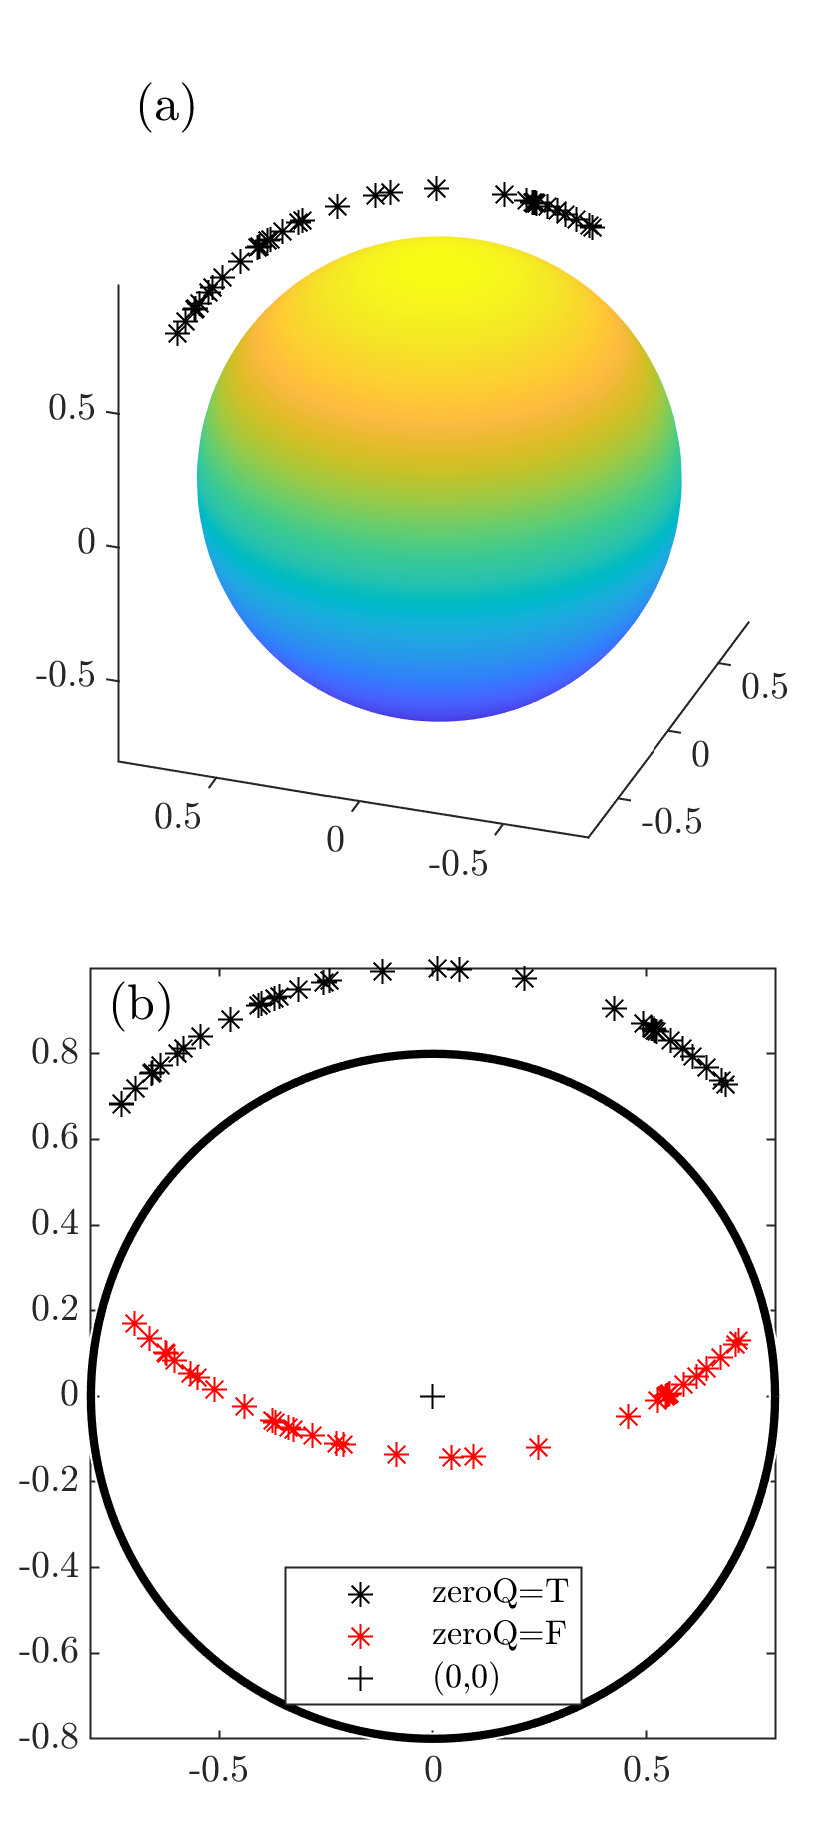
\includegraphics{bary-remove-deg.png}
    \caption{3D Cartesian to 2D Cartesian analogue of 8D Cartesian to 7D Cartesian degeneracy removal used in barycentric interpolation approach. Starting spherical arc points on surface of 2-sphere (a) and degenerate dimension removed via \acrlong{svd} projection to 2D Cartesian (b) with either the origin (black plus) preserved (black asterisks, \textit{zeroQ=T}) or ignored (red asterisks, \textit{zeroQ=F}). The sphere (a) and circle (b) each have a radius of 0.8 and are used as a visualization aid only.}
    \label{fig:bary-remove-deg}
\end{figure}

\begin{figure}
    \centering
    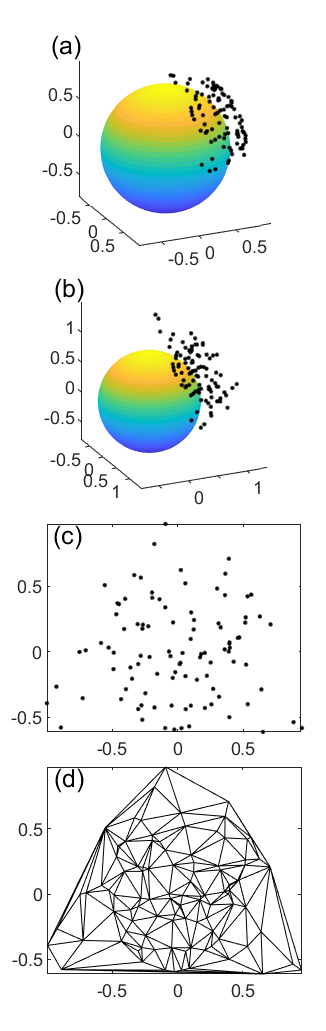
\includegraphics{bary-delaunay.png}
    \caption{3D Cartesian to 2D Cartesian analogue of 7D Cartesian to 6D Cartesian mesh triangulation used in barycentric interpolation approach. Normalized starting points on surface of 2-sphere (a), points projected onto hyperplane tangent to mean of starting points (b), degenerate dimension removed via \acrlong{svd} projection to 2D Cartesian (c), and Delaunay triangulation in 2D Cartesian (d). The sphere in (a) and (b) has a radius of 0.8 and is used as a visualization aid only.}
    \label{fig:bary-delaunay}
\end{figure}

There are approximately 1900 facets per point, 7 vertices per facet, and \num{1e8} total facets for a \num{50000} point mesh in 7D Cartesian. Due to the large number of facets per point of a high-dimensional, spherical, simplex-based triangulation and for computational speed, a given prediction point intersection within the input mesh is determined by considering facets connected to up to some number of \glspl{nn} in the mesh (in this work, 10 \glspl{nn}) for a given prediction point. In cases where an intersecting facet is not found in these connected facets due to high-aspect ratio facets or prediction point falling outside the mesh within a given tolerance, \gls{nn} interpolation and extrapolation are used, respectively, with an identical implementations for either interpolation or extrapolation given in \cref{sec:methods:nn}.

\subsubsection{Interpolation via Barycentric Coordinates}

Once barycentric coordinates are computed for a prediction point within the input mesh, the interpolated value is found by taking the dot product of the barycentric coordinates and the properties of the corresponding vertices of the intersecting facet via
\begin{equation}
v=\underset{i=1}{\overset{N}{\sum }}\lambda _i v_i
\end{equation}
where $\lambda$, $v$, $v_i$ and $N$, are the barycentric coordinates, interpolated property, property of the $i$th vertex of the intersecting facet, and number of vertices in a given facet ($N = 7$ for the degeneracy-free 6-sphere).
    
\subsection{Gaussian Process Regression or Kriging} \label{sec:methods:gpr}

The implemented \gls{gpr} scheme uses MATLAB's built-in function, \texttt{fitrgp} with default parameters in MATLAB R2020b except for \texttt{PredictMethod}, which is set to \texttt{'exact'} regardless of the number of input points. For a general treatment of \gls{gpr}, see \cite{rasmussenGaussianProcessesMachine2006}. A number of non-default settings -- \texttt{FitMethod}, \texttt{PredictMethod}, \texttt{OptimizeHyperarameters}, and \texttt{ActiveSetMethod} -- were tested and resulted in marginal error improvement relative to results produced by the default parameters which usually also resulted in a deficit in time performance; however, custom \texttt{fitrgp} options can still be passed into \texttt{interp5DOF} \cite{bairdFiveDegreeofFreedom5DOF2020}. For faster, less accurate, and less memory-intensive computations consider using \gls{fic} (\texttt{'fic'}) approximation as the \texttt{PredictMethod} instead. % as summarized in the table below.

% \item MATLAB fitrgp
%         \begin{enumerate}
%             \item squared exponential covariance function
%             \item bcd fit method (others are sd, fic etc.)
%             \item constant basis function
%             \item exact or bcd predict methods (also fic)
%             \item quasi-newton optimizer
%             \item optimize KernelScale and Sigma hyperparameters with bayesopt Optimizer
%             \item ActiveSetMethod - entropy (others, log likelihood, sparse greedy approximation)
%         \end{enumerate}

\subsection{Inverse-Distance Weighting} \label{sec:methods:idw}

A simple \gls{idw} approach is implemented similar to a MATLAB \gls{fex} submission \cite{tovarInverseDistanceWeight2020}. A pairwise distance matrix is computed and distances outside of a specified radius $r$ are ignored, and $r$ given by a scaled version of the mean of the \gls{nn} pairwise Euclidean distance matrix: 
\begin{equation}
r=\sqrt{2} \mu
% r=\frac{\mu }{\sqrt{2}}
% r=\frac{\sum _{k=1}^N \sum _{j=1}^N \sqrt{\sum _{i=1}^N \left(x_{i,j}-x_{i,k}\right){}^2}}{\sqrt{2} N},j\neq k
% where $r$, $x_{i,j}$, $x_{i,k}$, and $N$ represent the radius of influence, $i$th component of the $j$th point, $i$th component of the $k$th point, and total number of points, respectively.
\end{equation}
where $r$ and $\mu$ represent the radius of influence and mean \gls{nn} distance, respectively. Euclidean distance is used by default to define the weight matrix via $W_{i,j} = \frac{1}{D_{i,j}^L}$, where $i,j$ gives the $i$th row and $j$th column and $W$, $D$, and $L$ represent the weight matrix, pairwise-distance matrix, and norm-power (i.e. $L = 2$ for Euclidean), respectively. For prediction points that have no input mesh points within the specified radius, the \gls{nn} approach is used instead (\cref{sec:methods:nn}). The rest of the interpolated prediction point values are computed normally using \gls{idw} as described.

\subsection{Nearest Neighbor} \label{sec:methods:nn}

\Gls{nn} is one of the simplest interpolation schemes implemented using the built-in MATLAB function \texttt{dsearchn}. Euclidean distance will produce the same results as octonion distance for this method. \Gls{nn} computations are fast due to the simple calculation of Euclidean distance and ability to use optimized, built-in methods.

\subsection{Random Grain Boundary Sampling} \label{sec:methods:rand}

Random sampling of \glspl{gb} occurs in \gls{5dof} space by taking a random, cubochorically sampled quaternion and random unit vector \gls{bp} normal as a pair and then converting from this \gls{5dof} representation to a \gls{gbo}. All random sampling of octonions reported in this work take place via this scheme.

% \begin{enumerate}
    
    % \item Gaussian process regression
    % \begin{enumerate}
        
    % \end{enumerate}
    
% \end{enumerate}

\section{Results and Discussion} \label{sec:results}

To illustrate the utility of the \gls{cmo} framework for one application, namely interpolation, we compare the (i) accuracy, and (ii) efficiency of the four previously described interpolation methods implemented over the pFZ with each other and with existing methods from the literature (see \cref{sec:intro}).

For these tests, we used the 5DOF GB energy function developed by Bulatov, Reed and Kumar [REF], as the test function. We first generated a pFZ triangulation containing \num{50000} GBO vertices, corresponding to an average mesh resolution of about \SI{2.87}{\degree.} (see \cref{fig:nndist}). We denote this set of GBs by \texttt{gb\_v}. The test function was then evaluated at each of these points and the values were stored in the vector \texttt{f\_v}. We then generated \num{10000} GBO query points, denoted by \texttt{gb\_q}. Finally, we used \texttt{interp5DOF()} to predict the function value at the query points, which were stored in the vector \texttt{f\_q}. We also evaluated the test function at the query points to obtain the true function values, \texttt{f\_true}. We repeated this process for each of the interpolation methods, and compared the predictions, \texttt{f\_q}, to the true values, \texttt{f\_true}.
\begin{figure}
\centering
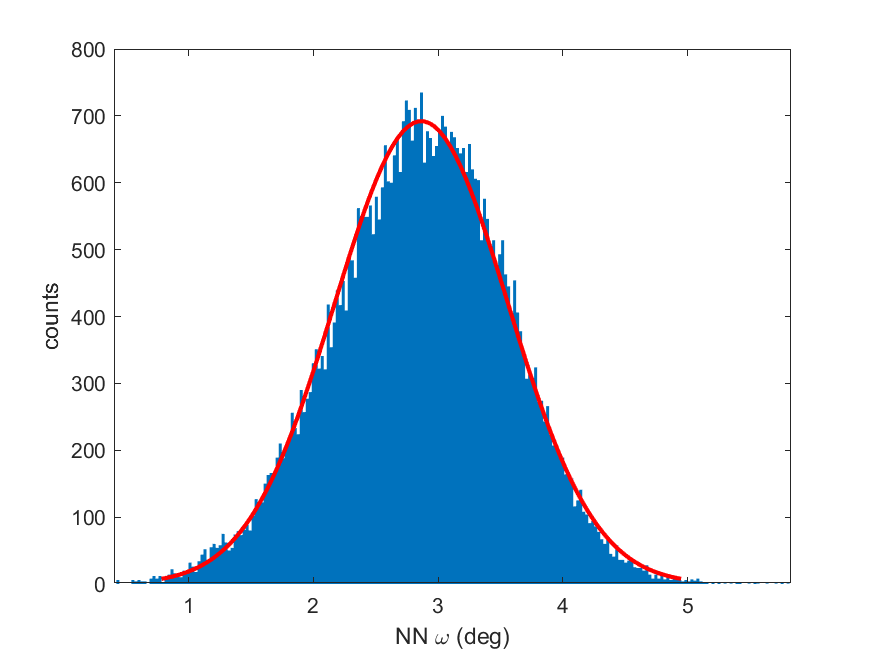
\includegraphics[width=0.5\linewidth]{disthist50000.png}
\caption{Histogram of \acrlong{nn} octonion distances ($\omega$) for the vertices of the pFZ triangulation used for testing. The mean and standard deviation are \SI{2.87}{\degree} and \SI{0.7}{\degree}, respectively.}
\label{fig:nndist}
\end{figure}

\subsection{Interpolation Accuracy}
\label{sec:results:accuracy}

\Cref{fig:brkparity50000} provides hexagonally binned parity plots \cite{beanHexscatter2020} for each of the four interpolation methods.
\begin{figure}
    \centering
    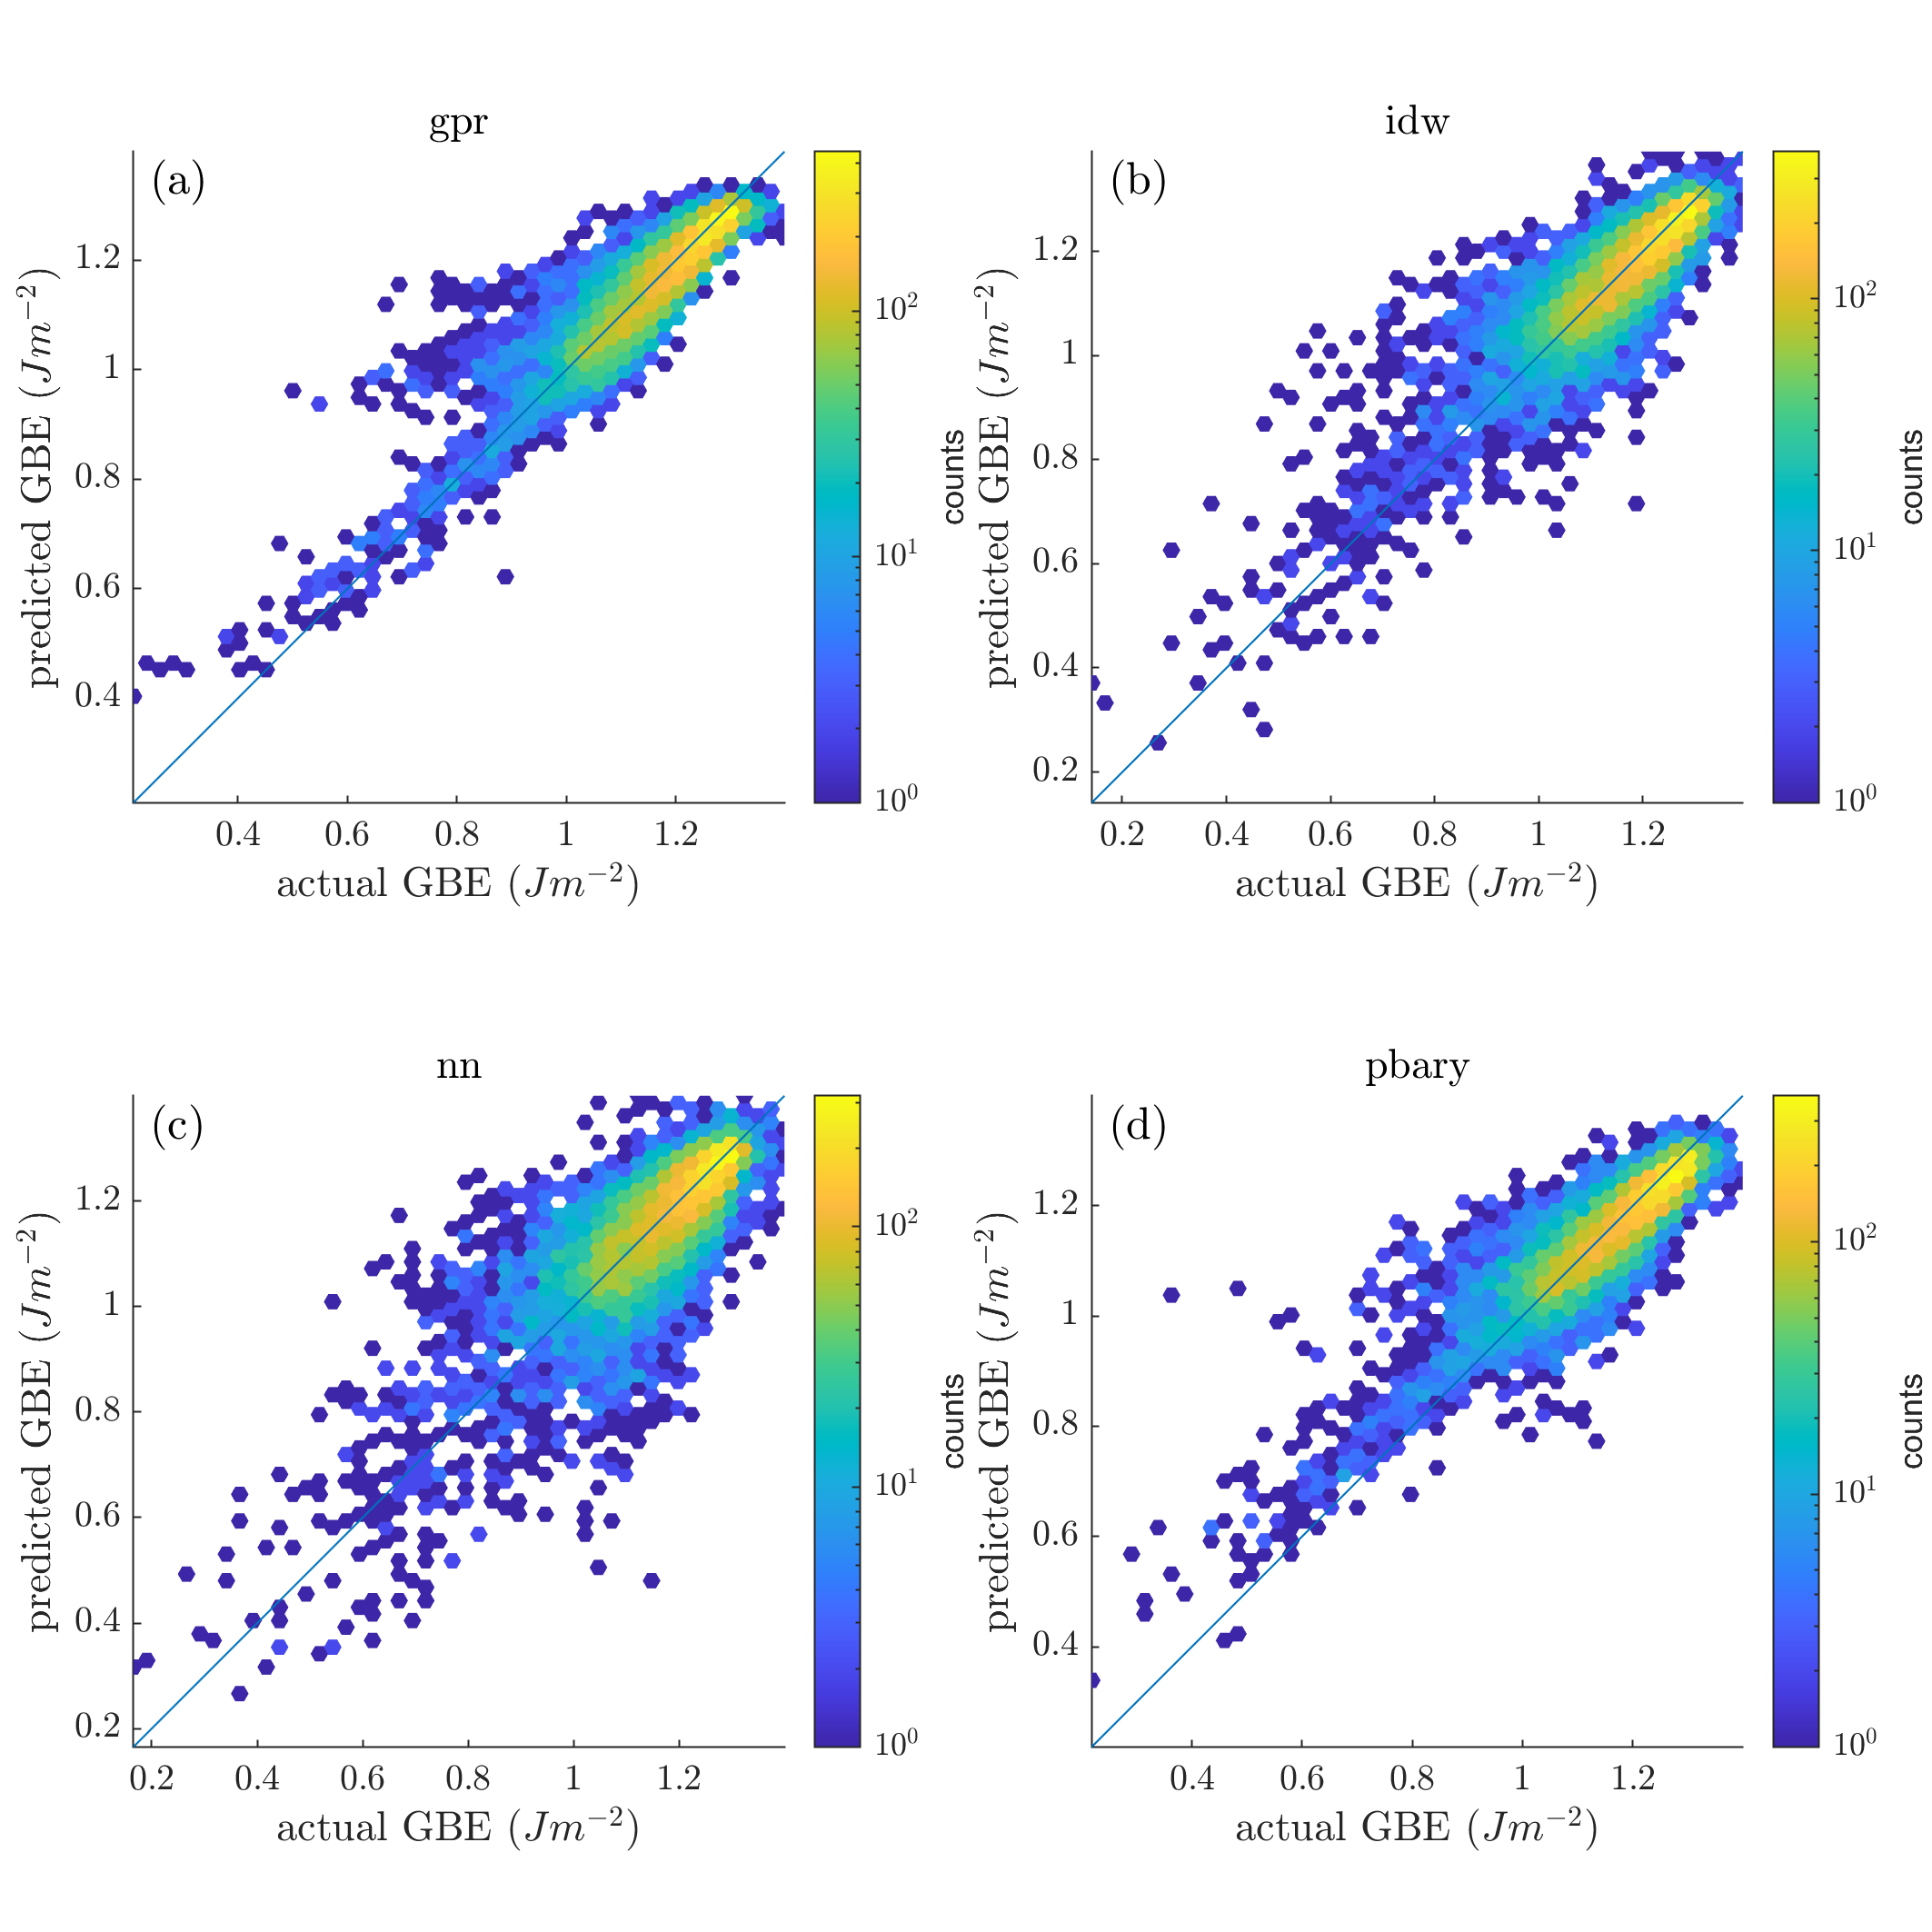
\includegraphics[width=0.75\linewidth]{brkparity50000.png}
    \caption{Hexagonally binned parity plots for 50000 mesh and 10000 prediction octonions formed via pairs of a random cubochorically sampled quaternion and a spherically sampled random boundary plane normal. Interpolation via (a) \acrlong{gpr}, (b) \acrlong{idw}, (c) \acrlong{nn}, (d) and barycentric coordinates.  \acrlong{brk} \acrlong{gbe} function for \gls{fcc} Ni was used as the test function.}
    \label{fig:brkparity50000}
\end{figure}

All of the methods permit successful interpolation, and the highest density region in all cases falls squarely on the parity line. The \Gls{gpr} and barycentric results show a slight asymmetry such that low energy values are overpredicted more often than they are underpredicted. The width of the point clouds provides a qualitative indication of the dispersion in the prediction errors. Quantitative measures of the overall accuracy are presented in \cref{tab:rmse-error-comparison} and \cref{tab:mae-error-comparison}.

\begin{table}
\caption{Comparison of average interpolation error for each interpolation method in the present work, using \num{50000} points in the definition of the pFZ. Comparison to the work of other authors is also included. A constant model, whose value was chosen to be the mean of \texttt{f\_v}, was used as a control.}
\centering
\begin{tabular}{lccc}
\toprule
Method                                                      & \multicolumn{1}{l}{\# \glspl{gb}} & \multicolumn{1}{l}{\gls{rmse} (\SI{}{\J\per\square\meter})} & \multicolumn{1}{l}{Cst, Avg \gls{rmse} (\SI{}{\J\per\square\meter})} \\ \midrule
\Gls{gpr}                                                   & \num{50000}                       & \num{0.0541}                                                & \num{0.1296}                                                         \\
Barycentric                                                 & \num{50000}                       & \num{0.0607}                                                & \num{0.1296}                                                         \\
\gls{idw}                                                   & \num{50000}                       & \num{0.0680}                                                & \num{0.1296}                                                         \\
\gls{nn}                                                    & \num{50000}                       & \num{0.0821}                                                & \num{0.1296}                                                         \\
\gls{lobpcg} \cite{shenDeterminingGrainBoundary2019}        & \num{180000}                      & \num{0.0076}--\num{0.0277}                                  & \num{0.0976}                                                         \\
\gls{ann} \cite{echeverrirestrepoUsingArtificialNeural2014} & \num{17176}                       & N/A                                                         & \num{0.0854}                                                         \\
\gls{lkr} \cite{chesserLearningGrainBoundary2020}           & \num{388}                         & \num{0.0977}                                                & \num{0.2243}                                                         \\ \bottomrule
\end{tabular}
\label{tab:rmse-error-comparison}
\end{table}

% \begin{table}
% \caption{Comparison of average interpolation error for each interpolation method in the present work, using \num{50000} points in the definition of the pFZ. Comparison to the work of other authors is also included. A constant model, whose value was chosen to be the mean of \texttt{f\_v}, was used as a control.}
% \centering
% \begin{tabular}{lccc}
% \toprule
% Method                                                & \multicolumn{1}{l}{\# \glspl{gb}} & \multicolumn{1}{l}{Cst, Avg \gls{mae} (\SI{}{\J\per\square\meter})} & \multicolumn{1}{l}{\gls{mae} (\SI{}{\J\per\square\meter})} \\ \midrule
% \Gls{gpr}                                             & \num{50000}                       & \num{0.0964}                                                        & \num{0.0372}                                               \\
% Barycentric                                           & \num{50000}                       & \num{0.0964}                                                        & \num{0.0418}                                               \\
% \gls{idw}                                             & \num{50000}                       & \num{0.0964}                                                        & \num{0.0470}                                               \\
% \gls{nn}                                              & \num{50000}                       & \num{0.0964}                                                        & \num{0.0573}                                               \\
% LOBPCG \cite{shenDeterminingGrainBoundary2019}        & \num{180000}                      & \num{0.0466}                                                        & N/A                                                        \\
% ANN \cite{echeverrirestrepoUsingArtificialNeural2014} & \num{17176}                       & \num{0.0617}                                                        & \num{0.0486}--\num{0.085}                                  \\
% LKR \cite{chesserLearningGrainBoundary2020}           & \num{388}                         & \num{0.1752}                                                        & \num{0.0977}                                               \\ \bottomrule
% \end{tabular}
% \label{tab:mae-error-comparison}
% \end{table}

\begin{table}
\caption{Comparison of average interpolation error for each interpolation method in the present work, using \num{50000} points in the definition of the pFZ. Comparison to the work of other authors is also included. A constant model, whose value was chosen to be the mean of \texttt{f\_v}, was used as a control.}
\centering
\begin{tabular}{lccc}
\toprule
Method                                                      & \multicolumn{1}{l}{\# \glspl{gb}} & \multicolumn{1}{l}{\gls{mae} (\SI{}{\J\per\square\meter})} & \multicolumn{1}{l}{Cst, Avg \gls{mae} (\SI{}{\J\per\square\meter})} \\ \midrule
\Gls{gpr}                                                   & \num{50000}                       & \num{0.0372}                                               & \num{0.0964}                                                        \\
Barycentric                                                 & \num{50000}                       & \num{0.0418}                                               & \num{0.0964}                                                        \\
\gls{idw}                                                   & \num{50000}                       & \num{0.0470}                                               & \num{0.0964}                                                        \\
\gls{nn}                                                    & \num{50000}                       & \num{0.0573}                                               & \num{0.0964}                                                        \\
\gls{lobpcg} \cite{shenDeterminingGrainBoundary2019}        & \num{180000}                      & N/A                                                        & \num{0.0466}                                                        \\
\gls{ann} \cite{echeverrirestrepoUsingArtificialNeural2014} & \num{17176}                       & \num{0.0486}--\num{0.085}                                  & \num{0.0617}                                                        \\
\gls{lkr} \cite{chesserLearningGrainBoundary2020}           & \num{388}                         & \num{0.0977}                                               & \num{0.1752}                                                        \\ \bottomrule
\end{tabular}
\label{tab:mae-error-comparison}
\end{table}

\begin{table}
\caption{Comparison of average interpolation error for each interpolation method in the present work, using \num{50000} points in the definition of the pFZ. Comparison to the work of other authors is also included. A constant model, whose value was chosen to be the mean of \texttt{f\_v}, was used as a control.}
\centering
\begin{tabular}{lccc}
\toprule
Method & \# \glspl{gb} & Runtime (\SI{}{\second}) \\
\midrule
\Gls{gpr} & x & x \\
Barycentric & x & x \\
\gls{idw} & x & x \\
\gls{nn} & x & x \\
Constant & 0.13 & 0.097 \\
LOBPCG \cite{shenDeterminingGrainBoundary2019} & 0.01--0.03 & --- \\
ANN \cite{echeverrirestrepoUsingArtificialNeural2014} & --- & 0.05--0.09 \\
LKR \cite{chesserLearningGrainBoundary2020} & 0.0977 & --- \\
\bottomrule
\end{tabular}
\label{tab:runtime-comparison}
\end{table}

To aid in objective interpretation of the error metrics, comparison is made to a constant valued control model, whose value is chosen to be the average of \texttt{f\_v} (approximately \SI{1.16}{\J\per\square\meter} in the limit of $nmeshpts \rightarrow \infty$) resulting in \gls{rmse} and \gls{mae} values of approximately \num{0.130} and \SI{0.097}{\J\per\square\meter}.

Of the four interpolation methods from this work, \Gls{gpr} has the lowest error, both in terms of \gls{rmse} and \gls{mae}, while \Gls{nn} has the highest error. ... Add comments comparing the performance of the methods in \cref{tab:error-comparison} to the constant value and the literature methods. This is where we highlight that your method outperforms prior work.

The accuracy of the predictions made using the pFZ methods depends on the resolution of the pFZ triangulation. \Cref{fig:brkerror} compares the prediction accuracy for each of the 4 methods to the constant valued control model, as a function of the number of mesh vertices (\texttt{nmeshpts}). As expected, higher resolution triangulations result in lower error and diminishing returns (\cref{fig:brkerror}). Moreover, the standard deviations produced via multiple runs are tightly constrained and generally shrink as the mesh size increases. 

\Gls{gpr} consistently gives lower error than the other three interpolation methods. It is interesting to see that despite qualitative differences in the parity plots for barycentric and \gls{idw} interpolation, these two methods produce similar \gls{rmse} and \gls{mae} values. \Gls{nn} interpolation produces the worst error of the four methods, but is better than the constant valued control model above several hundred mesh points. 

Both \gls{gpr} and \gls{idw} seem to reach a plateau near 20,000 mesh points. It is worthwhile to note that both of these methods are kernel-based in that a model parameter controls the size of the region that can influence the interpolation results. In the \gls{gpr} case, this is automatically calculated. In the \gls{idw} case, this is set to a constant value independent of the mesh size. It is likely that better tuning of the kernel parameters in these two methods could further decrease the obtained errors. By contrast, barycentric interpolation automatically adjusts its effective region of influence because the size of the simplices in the mesh decreases as the number of vertices increases.
\begin{figure}
    \centering
    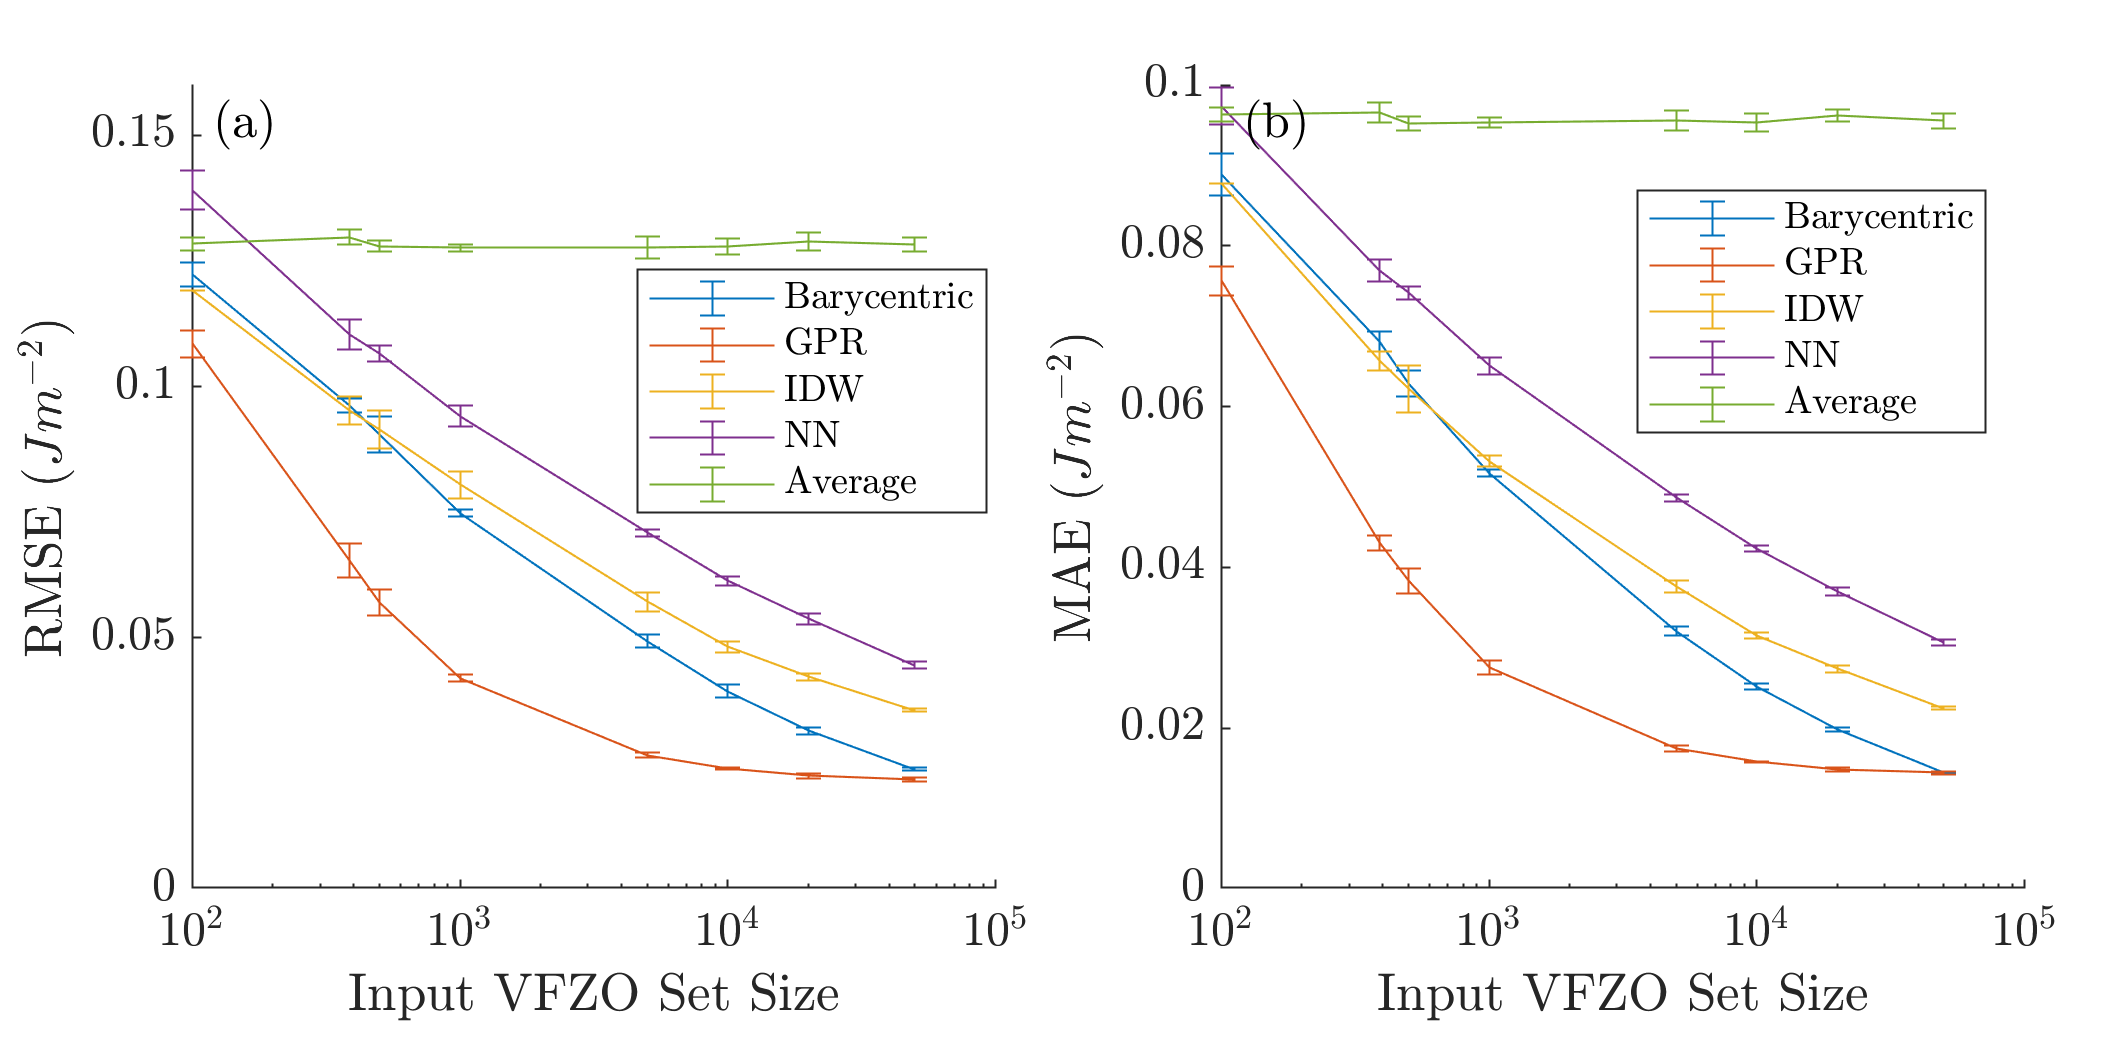
\includegraphics[width=0.5\linewidth]{brkerror.png}
    \caption{Average \acrlong{rmse} and average \acrlong{mae} vs. number of mesh points for barycentric (blue), \acrlong{gpr} (\acrshort{gpr}) (orange), \acrlong{idw} (\acrshort{idw}) (yellow), and \acrlong{nn} (\acrshort{nn}) (purple) interpolation for approximately 10 random runs with different mesh and prediction points. Standard deviations of approximately 10 runs are also included. Compare with approximately \SI{0.13}{\J\per\square\meter} and \SI{0.95}{\J\per\square\meter} \acrshort{rmse} and \acrshort{mae}, respectively, for a constant model using the average of the mesh properties (approximately \SI{1.16}{\J\per\square\meter}).}
    \label{fig:brkerror}
\end{figure}

\subsection{Interpolation Efficiency}
\label{sec:results:efficiency}

\Gls{gpr} is fast and has lower error compared to barycentric interpolation; however, the entire process has to be rerun (in current implementation) if the responses or the predictors change.

Barycentric interpolation is fast once the triangulation is computed. In other words, it is fast even if responses (i.e. \glspl{gbe}) change, but needs to be recomputed if the predictors (i.e. \glspl{gb}) change.

Computational runtimes of the various interpolation methods are also shown (\cref{fig:runtime}). Barycentric interpolation takes the longest, which is compounded by the fact that it is the only parallelized method by default (not accounted for in \cref{fig:runtime}). In other words, since 12 cores were used to obtain these runtime results, the total runtime across all cores is much higher compared with the other methods; however, it is possible that other methods used multi-threading via built-in vectorized functions. The long computation times result primarily from the large number of facets present in a high-dimensional mesh triangulation and the interconnectedness of facets with respect to each other. \Gls{gpr} is the second-longest in terms of of runtime, but produces better error than any of the other three methods. \Gls{nn} and \gls{idw} interpolation have vectorized implementations and are much simpler than the barycentric and \gls{gpr} methods. Consistent with expectations, \gls{nn} and \gls{idw} exhibit almost negligible runtimes; however, this is at the expense of error trade-offs discussed earlier (\cref{sec:results:mdlerror}). It should also be noted that barycentric interpolation and \gls{gpr} have much higher memory requirements than \gls{nn} and \gls{idw} due to the need to store large matrices (unless \textit{fitrgp Predict Method = \gls{fic}}). Because the default implementation of \gls{idw} uses a radius cut-off, the distance and weight matrices can be stored as sparse objects, dramatically reducing both the storage requirements and computational complexity of this method. We expect that a \gls{knn} approach would produce similar results both in terms of runtime and error when a relatively uniform sampling of \gls{gbc} is obtained.

\begin{figure}
    \centering
    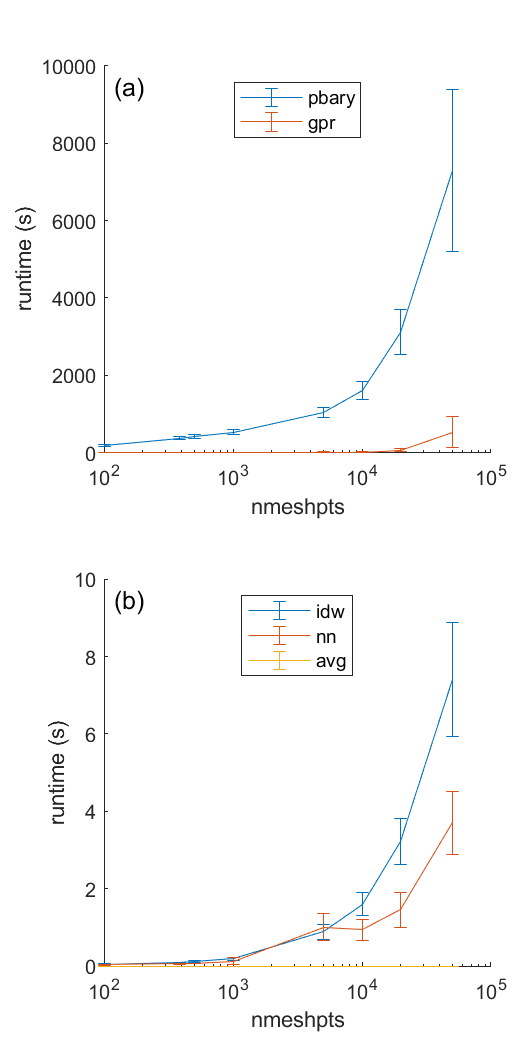
\includegraphics{runtime.png}
    \caption{
    Average runtime (s) and standard deviation (approximately 10 runs) vs. number of mesh points for barycentric (a, blue) and \acrlong{gpr} (\acrshort{gpr}) (a, orange), \acrlong{idw} (\acrshort{idw}) (b, blue), \acrlong{nn} (\acrshort{nn}) (b, orange) interpolation using 12 cores compared against runtime (s) for an average model (b, yellow). Because \acrshort{gpr}, \acrshort{idw}, and \acrshort{nn} method defaults do not use parfor loops but may have internal multi-core vectorization, it is unclear to what extent the number of cores affects the runtime of methods other than barycentric interpolation. \Acrlong{gb} symmetrization runtime was not included; however, symmetrization takes approximately one minute on 6 cores (Intel i7-10750H, 2.6 GHz) and is a common step in every interpolation method (i.e. it is fundamental to the \acrlong{cmo} framework).
    %Runtime (s) vs. number of mesh points for barycentric (blue), \acrlong{gpr} (\acrshort{gpr}) (orange), \acrlong{idw} (\acrshort{idw}) (yellow), and \acrlong{nn} (\acrshort{nn}) (purple) interpolation using 12 cores. Because \acrshort{gpr}, \acrshort{idw}, and \acrshort{nn} method defaults do not use parfor loops but may have internal multi-core vectorization, it is unclear to what extent the number of cores affects the runtime of methods other than barycentric interpolation. \Acrlong{gb} symmetrization runtime was not included; however, symmetrization takes approximately one minute on 6 cores (Intel i7-10750H, 2.6 GHz) and is a common step in every interpolation method (i.e. it is fundamental to the \acrlong{cmo} framework).
    }
    \label{fig:runtime}
\end{figure}

\section{Conclusion} \label{sec:conclusion}

A high fidelity \gls{cmo} framework for interpolation of \gls{gb} properties is presented and four interpolation schemes built on the \gls{cmo} framework are described and tested. This framework enables faster computation of pairwise distance matrices and produces lower error than previous methods.
%similar error to a machine learning approach that does not consider symmetrically equivalent \glspl{gb} \cite{echeverrirestrepoUsingArtificialNeural2014}.
Barycentric, \gls{gpr}, and \gls{idw} always yield lower error than pure \gls{nn} interpolation (\cref{fig:brkparity50000}), especially for large mesh sizes. The approach is general to any crystal system (which can be selected by the parameter \texttt{pgnum}). \Gls{gpr} is demonstrated to offer a competitive advantage in computation time and error relative to other methods considered in this work. It is the the generally recommended interpolation method for the \gls{cmo} framework; however, the other approaches can meet other, niche needs.
    
\subsection{Future Work} \label{sec:conclusions:future}

\subsubsection{\glsentrytitlecase{fz}{long}}
It is unclear how difficult it would be to define \gls{fz} borders with high-symmetry GBs on the perimeter, and it is possible that the borders would exhibit curvature. Ideally, a convex hull of the points that define such a border would also define a \gls{fz}; however, if the borders have curvature, this is not guaranteed. An additional advantage of the \gls{cmo} framework is the possibility of defining discontinuous or "sharp" features within a closed-mesh using existing methods such as in \cite{tianNonUniformSubdivisionSurfaces2020}. Because high-symmetry \glspl{gb} can be sampled via knowledge of misorientation and \gls{bp} \glspl{fz} and may even have generalized, analytical representations in octonion space, such an approach has great potential to increase interpolation accuracy of methods built on the \gls{cmo} framework (especially near high-symmetry grain boundaries). Exaggerated errors may also arise for \glspl{gb} near the low-symmetry exterior of the mesh. In lieu of defining every \gls{seo} of every mesh point, ensemble methods can be employed to combat these interpolation inaccuracies. We think it is reasonable to expect that a low number of components in an ensemble (e.g. 8) could negate exaggerations in errors near mesh-exteriors. For example, instead of using a single reference octonion, a low number of reference octonions with maximized pairwise-distances \cite{dolanBenchmarkingOptimizationSoftware2004,ConstrainedElectrostaticNonlinear2020} with respect to each other can define multiple meshes and ensure that every \gls{gb} is situated reasonably far from the mesh exterior for at least one mesh in the ensemble. It may be necessary to first explore the source of error bias (Section \cref{results:general:bias}) to verify that higher error preferentially occurs near the \gls{fz} exterior.

\subsubsection{Other Interpolation Methods}
Including an ensemble approach described above, other options for continuing this work involve extending linear interpolation methods to hyperspherical spline interpolation \cite{taijeronSplineInterpolationSmoothing1994}. Unfortunately, built-in MATLAB spline interpolations require gridded (as opposed to scattered) data in high dimensions (four or higher in \textit{spapi} and \textit{interpn}), so an alternative implementation is likely required. A gridded mesh could be defined; however, due to the curse-of-dimensionality and the fact that \glspl{gbo} are on the surface of a hypersphere, an unreasonably large number of points compared to the methods described here and/or an \gls{svd} projection to 6D Cartesian (neither distance- nor angle-preserving) would likely be required. Generalized barycentric coordinates \cite{floaterGeneralizedBarycentricCoordinates2015,meyerGeneralizedBarycentricCoordinates2002,langerSphericalBarycentricCoordinates2006} are another implementation option which could potentially speed up and improve error in barycentric interpolation time since the number of vertices per facet can increase. It is also likely that for large mesh sizes (e.g. \num{10000}+ mesh points), an \gls{ann} approach \cite{echeverrirestrepoUsingArtificialNeural2014} could also decrease interpolation error while maintaining low computation times. Further optimization of hyperparameters used in this work, such as for noise standard deviation and smoothness length in \gls{gpr} may lead to lower model error.

\subsubsection{Other \glsentrytitlecase{gb}{long} Distance Metrics}
Barycentric interpolation using other \gls{gb} distance metrics \cite{morawiecDistancesGrainInterfaces2019} could also be performed by recomputing barycentric coordinates in a \gls{cmo} triangulation, supplying octonion facet vertices to a simplex reconstruction using only edge lengths computed by the alternative distance metric \cite{connorHighdimensionalSimplexesSupermetric2017}, or by computing a manifold from only a pairwise distance matrix \cite{boissonnatOnlyDistancesAre2017}.

\subsubsection{Applications}
We think it is straightforward to apply these methods to restricted regions of \gls{5dof} space. In addition to interpolations involving \gls{gbe}, \gls{gbcd} (i.e. similar to fitting a curve to a histogram) and other \gls{gb} properties such as diffusivity and mobility could also be interpolated. Finally, linking this interpolation scheme with polycrystal data such as 3D microstructural \gls{tj} datasets (e.g. Ni \cite{liRelativeGrainBoundary2009}) via \textit{TJ2GBE} \cite{shenDeterminingGrainBoundary2019} or similar approaches geared towards large datasets is particularly intriguing.


% \section{Supplemental}
% \begin{enumerate}
%     \item conversion from octonion to \gls{5dof}
%     \item high-aspect ratio facets
%     \item facet subdivision
%     \item spherical vs. planar barycentric interpolation
%     \item tolerances of interpolation and intersecting facets
%     \item non-intersection percentage vs. number of mesh points
%     \item "excess" arc length in pairwise distance matrices
%     \begin{enumerate}
%         \item gradient optimization and global optimization of U(1) twist symmetry with marginal improvement
%     \end{enumerate}
%     \item identification and subdivision of hull exterior
%     \item distribution of data in \gls{mfz} and \gls{bp} spaces
%     \item comments on \gls{gpr} hyperparameters
% \end{enumerate}

\newpage
\printglossaries
%need to manually clear cached files & logs in overleaf to get new abbreviations to appear

\newpage
\bibliographystyle{elsarticle-num-names}
\bibliography{5dof-gb-energy.bib}



\end{document}
